%% 
%% Copyright 2007-2024 Elsevier Ltd
%% 
%% This file is part of the 'Elsarticle Bundle'.
%% ---------------------------------------------
%% 
%% It may be distributed under the conditions of the LaTeX Project Public
%% License, either version 1.3 of this license or (at your option) any
%% later version.  The latest version of this license is in
%%    http://www.latex-project.org/lppl.txt
%% and version 1.3 or later is part of all distributions of LaTeX
%% version 1999/12/01 or later.
%% 
%% The list of all files belonging to the 'Elsarticle Bundle' is
%% given in the file `manifest.txt'.
%% 
%% Template article for Elsevier's document class `elsarticle'
%% with harvard style bibliographic references

\documentclass[preprint,12pt]{elsarticle}

%% Use the option review to obtain double line spacing
%% \documentclass[preprint,review,12pt]{elsarticle}

%% Use the options 1p,twocolumn; 3p; 3p,twocolumn; 5p; or 5p,twocolumn
%% for a journal layout:
%% \documentclass[final,1p,times]{elsarticle}
%% \documentclass[final,1p,times,twocolumn]{elsarticle}
%% \documentclass[final,3p,times]{elsarticle}
%% \documentclass[final,3p,times,twocolumn]{elsarticle}
%% \documentclass[final,5p,times]{elsarticle}
%% \documentclass[final,5p,times,twocolumn]{elsarticle}

%% For including figures, graphicx.sty has been loaded in
%% elsarticle.cls. If you prefer to use the old commands
%% please give \usepackage{epsfig}
\graphicspath{{plots}}

%% The amssymb package provides various useful mathematical symbols
\usepackage{amssymb}
%% The amsmath package provides various useful equation environments.
\usepackage{amsmath}
%% The amsthm package provides extended theorem environments
%% \usepackage{amsthm}

%% NOTE these packages were not in the original template
\usepackage{tabularx}
\usepackage{lscape}
\usepackage{empheq}
\usepackage{todonotes}
\usepackage{makecell}

\biboptions{sort&compress}

%% The lineno packages adds line numbers. Start line numbering with
%% \begin{linenumbers}, end it with \end{linenumbers}. Or switch it on
%% for the whole article with \linenumbers.
\usepackage{lineno}
\linenumbers

\journal{Ecological Modelling}

\usepackage[colorlinks=true]{hyperref}


\begin{document}

\begin{frontmatter}

%% Title, authors and addresses

%% use the tnoteref command within \title for footnotes;
%% use the tnotetext command for theassociated footnote;
%% use the fnref command within \author or \affiliation for footnotes;
%% use the fntext command for theassociated footnote;
%% use the corref command within \author for corresponding author footnotes;
%% use the cortext command for theassociated footnote;
%% use the ead command for the email address,
%% and the form \ead[url] for the home page:
\title{
    Predictive modelling of chemical mixture toxicity to amphibians in \textit{Discoglossus galganoi}
    larvae and metamorphs
    }
%% \tnotetext[label1]{}
\author[UOS]{Simon Hansul}
%% \ead{email address}
%% \ead[url]{home page}
%% \fntext[label2]{}
%% \cortext[cor1]{}
%% \affiliation{organization={},
%%             addressline={},
%%             city={},
%%             postcode={},
%%             state={},
%%             country={}}
\author[UCLM]{Samuel González-López}
\author[UCLM]{Manuel E. Ortiz-Santaliestra}
\author[EFSA]{Jean Lou CM Dorne}
\author[UOS]{Andreas Focks}
%
\affiliation[UOS]{Institute of Mathematics, Universit\"ät Osnabr\"uck}
\affiliation[UCLM]{Institute for Game and Wildlife Research, University Castilla-La Mancha}
\affiliation[EFSA]{European Food Safety Authority}
\title{} %% Article title


\author{} %% Author name

%% Author affiliation


%% Abstract
\begin{abstract}
%% Text of abstract
In natural environments, amphibians are exposed to individual chemical substances, and regularly also to mixtures of chemicals. 
At the same time, prospective risk assessment methods that account for exposure to mixtures across substances, 
species and environmental conditions are not implemented, partly because the experimental assessment of mixtures is extremely resource-intensive. 
Due to their specific life cycle, as well as susceptibility to anthropogenic and biological stressors, 
amphibians are of particular relevance for the environmental risk assessment of chemicals. 
Therefore, we set out to develop a model that can account for toxic effects of chemical mixtures in amphibians, specifically anurans, 
that integrates established toxicokinetic-toxicodynamic modelling principles with an amphibian-specific dynamic energy budget model (AmphiDEB-TKTD). 
We calibrated the AmphiDEB-TKTD model to single-substance toxicity data for Flupyradifurone and 2,4-D in Discoglossus galganoi larvae, 
and found that the model can reproduce observed effects on larval growth and metamorphosis traits. 
Also, we could use the data to identify the underlying physiological modes of action (PMoA), 
since growth and timing of metamorphosis are differentially affected through different PMoAs. 
A cross-validation with data on effects at Gosner stage 46 further clarified the physiological mode of action, 
and demonstrated that effects on Gosner stage 46 can be predicted from effects on larvae up to Gosner stage 42, 
if an appropriate PMoA has been identified. Concerning binary mixture toxicity, 
the model correctly predicted a dominance effect of 2,4-D in a mixture with Flupyradifurone. 
This can be explained through the different PMoAs of Flupyradifurone (decrease in growth efficiency) and 2,4-D (increase in maintenance costs), 
which qualitatively differ in the severity of their effectsl, regarding the propagation to different apical endpoints. 
We conclude that the AmphiDEB-TKTD model appears as a practical tool for the risk assessment of chemical mixtures for anurans, 
while also being useful for the investigation of mechanisms of toxicity. 
Since the model has been validated on a substance combination of different PMoAs, 
further investigations should include the validation with substance combinations of identical PMoAs. 

\end{abstract}

%%Graphical abstract
\begin{graphicalabstract}
%\includegraphics{grabs}
\end{graphicalabstract}

%%Research highlights
\begin{highlights}
\item Toxicokinetic-toxicodynamic models were fitted to sublethal effect data of two pesticides in \textit{Discoglossus gagalnoi}
\item By integrating effects on growth and the timing of metamorphosis in the analysis, different physiological modes of action could be inferred for 2,4-D and Flupyradifurone
\item The effect on duration of metamorphosis can be predicted from the effects on larvae
\item 2,4-D exhibited a dominance effect in the binary mixture, which could be predicted from the single-substance effects.
\end{highlights}

%% Keywords
\begin{keyword}

\end{keyword}

\end{frontmatter}

\section{Introduction}
%
%context & need
Amphibians are currently not explicitly considered in the environmental risk assessment (ERA) of chemicals. 
It is rather assumed that assessments based on aquatic vertebrates (e.g. fish) 
and terrestric vertebrates (birds and mammals) are also protective for amphibians. 
While amphibian larvae are in fact often less sensitive to chemicals 
than amphibian aquatic stages \citep{weltjeCOMPARATIVEACUTECHRONIC2013}, 
this is not the case for all chemicals \citep{glabermanEvaluatingRoleFish2019}, 
and the process of metamorphosis represents a vulnverable point in the life-hisory of amphibians, 
which is not covered by using other vertebrates as proxies.\\
Furthermore, environmental exposure occurrs in mixtures. 
The relative effect of mixtures within the metamorphosis phase is so far largely unexplored, 
and it cannot be expected that mixture toxicity data will be generated for a wide range 
of species and chemicals, necessitating the development of predictive models.\\
%
% goal
In this study, we demonstrate the possible use of toxicokinetic-toxicodynamic (TKTD) models 
to support a reliable ERA of chemicals for amphibians, including the extrapolation 
of chemical effects from larvae to metamorphs and the prediction of mixture effects. 
In general, this approach aims to maximize the amount of knowledge gained 
from experimental data, 
and to minimize the need for future animal testing. \\
%
\subsection{Setting the scene: predictive modelling of chemical toxicity with Dynamic Energy Budgets}
%
Dynamic Energy Budget (DEB) models are by now the most established models 
for predictive and interpretable modelling of sublethal chemical toxicity 
\citep{jagerSimplifiedDynamicEnergy2012,martinExtrapolatingEcotoxicologicalEffects2013,sherborneModelingSublethalEffects2020,romoliEnvironmentalRiskAssessment2024}. 
These models describe the individual as a mass balance, 
starting with the amount of ingested food and ending with the central metabolic processes determining an 
individual's life-history:  
maintenance, growth, maturation and reproduction \citep{kooijmanDynamicEnergyBudget2010,jagerDEBkissQuestSimplest2013}.
DEB models can be extended to account for the idiosyncracies of the amphibian life cycle \citep{romoliDynamicEnergyBudget2024,hansulDynamicEnergyBudget2026}.
Effects of chemicals can be incorporated into DEB models by coupling them to a toxicokinetic-toxicodynamic (TKTD) submodel. 
These translate the external chemical exposure to an effect on the energy budgets, 
e.g. a decrease in a conversion efficiency, increase in maintenance costs or change in resource allocation.
\textit{A priori}, there is no good reason to deviate from 
the standard approach for the application to amphibians. 
In general, it can be necessary to include other PMoAs to explain 
observed effects, 
or to consider the simultaneous action of multiple PMoAs \citep{kochMakingSenseLifeHistory2021}.
While the toxicokinetic (TK) component can be expressed in different levels of detail, 
the most common approach in the context of DEB-TKTD models is a reduced TK submodule, where the external concentration is directly linked to an abstract quantity 
called scaled damage \citep{jagerRevisitingSimplifiedDEBtox2020}. 
The scaled damage is assumed to be proportional to a toxicologaically relevant internal concentration, 
but does not require measured internal concentrations to estimate the corresponding rate constants, 
since the rate at which scaled damge is accumulated or repaired is primarily linked to the dynamics of effects after exposure or non-exposure. 
The coupling of such a reduced TK module to a DEB model further allows to include feedbacks with growth and reproduction. 
While these are often included by default, it is also reasonable to start with the simplest possible model, i.e. exclude all feedbacks 
and evaluate \textit{a posteriori} whether a more complex model structure may be needed \citep{jagerRevisitingSimplifiedDEBtox2020,efsapanelonplantprotectionproductsandtheirresiduespprScientificOpinionState2018a}. 
% 
The application of DEB-TKTD models to the analysis of toxicity data has multiple advantages over a purely statistical approach \citep{jagerGoodReasonsBan2011,jagerItsTimeMoving2025}. 
For example, it allows to test hypotheses regarding the mechanisms through which a substance may affect the organism 
\citep{kochMakingSenseLifeHistory2021,weighmanUsingDynamicEnergy2023}. 
Based on such insights, the coupling to population models is possible \citep{jagerExtrapolatingToxicEffects2010,martinExtrapolatingEcotoxicologicalEffects2013}
and such approaches have been used to predict differences between individual-level and population-level sensitivity \citep{pereiraUnexpectedAbsenceNickel2019}, 
as well as mixture effects on the population level \citep{vlaeminckPredictingCombinedEffects2022}. Further relevant applications of DEB and DEB-TKTD models 
include the modelling of interspecific sensitivity with regards to apical endpoints \citep{zubrodBioQSARs20Unlocking2024} and prediction of effects 
under time-varying exposure \citep{romoliEnvironmentalRiskAssessment2024a}.
%
\subsection{Objective}
%
The objective of the present study was to test the applicability of DEB-TKTD models to 
analyze toxicity data in amphibians, specicially the anuran \textit{Discoglossus galganoi}, 
in order to draw conclusions about mechanisms of toxicity and synthesize effects 
on different endpoints and on different life stages. \\ 
We briefly describe and motivate the model structure, and report results on three case studies in \textit{D. galganoi}, 
concerning the estimation of DEB parameters from control data with account for biological variabiltiy,
the comparative effects of the herbicide 2,4 Dichlorphenoxyacetic acid (2,4-D) and the insecticide Flupyradifurone.
%
\section{Methods}
%
\subsection{Model description}
%
\subsubsection{Amphibian DEB model}
%
The DEB-TKTD model is based on DEBkiss \citep{jagerDEBkissQuestSimplest2013} 
and has been extended to account for amphibian metamorphosis \citep{hansulDynamicEnergyBudget2026}. 
In short, the model includes a metamorphic reserve compartment $E^{mt}$, 
which is defined as the amount of biomass that is used during metamorphosis to fuel 
maintenance costs and maturation. 
The parameter $\gamma$ determines the allocation of assimilated resources into the metamorphic reserve 
compartment. 
Under \textit{ad libitum} feeding conditions and at equilibrium, 
$\gamma$ is equal to the fraction of biomass that is reserve.\\
During metamorphosis, feeding rates decline and are assumed to reach 0 with the completion of metamorphosis. 
The decline in the size-specific feeding rate is coupled to the depletion of metamorphic reserves:
%
\begin{equation}
    \{ \dot{I} \}_{max}^{mt} = \{ \dot{I} \}_{max}^{lrv} \dfrac{E^{mt}}{E^{mt}_{max}}  
    \label{eq:dI_mt}
\end{equation}
%
Where  $\{ \dot{I} \}_{max}^{lrv}$ is the maximum size-spefific ingestion rate for larvae,
$\{ \dot{I} \}_{max}^{mt}$ is the current maximum size-spefific ingestion rate for metamorphs 
and $E^{mt}_{max}$ is the internally tracked maximum reserve level, 
reached at metamorphic climax.\\
By definition, metamorphosis is completed when the metamorphic reserve is depleted. 
The full dynamics of the model \citep{hansulDynamicEnergyBudget2026} are given by:
\begin{align}
    \dot{X}^{emb} &=
    \begin{cases}
        -\dot{I} & \text{if embryo} \\ 
        0 & \text{otherwise}
    \end{cases} \\
    \dot{X} &= 
    \begin{cases}
        0 & \text{if embryo} \\ 
        \dot{I} & \text{otherwise}
    \end{cases}\\
    \dot{I} &= 
    \begin{cases}
        0 & \text{if embryo} \\
        \{ \dot{I} \}_{\text{max}}\, f([X])\, S^{2/3} & \text{otherwise}
    \end{cases} \\
    \dot{A} &= y_A \eta_{IA} \dot{I} \\ 
    \dot{M} &= y_M k_M S \\ 
    \dot{J} &= y_M k_J H \\
    \dot{S} &= 
    \begin{cases}
        y_G \eta_{AS} (1-\gamma) (\kappa \dot{A} - k_M S) & \text{if larva} \\ 
        y_G \eta_{AS} \dot{A} & \text{if metamorph} \\
        y_G \eta_{AS} (\kappa \dot{A} - \dot{M}) & \text{otherwise}
    \end{cases} \\
    \dot{E}^{mt} &= 
    \begin{cases}
        y_G \eta_{AS} \gamma (\kappa \dot{A} - k_M S) & \text{if larva} \\
        -(\dot{M} + \dot{J} + \dot{H}) & \text{if metamorph} \\ 
        0 & \text{otherwise}
    \end{cases} \\
    \dot{H} &= 
    \begin{cases} 
        0 & \text{if adult} \\
        (1-\kappa) \dot{A} - \dot{J} & \text{otherwise} \\
    \end{cases} \\
    \dot{R} &= 
    \begin{cases} 
        y_R \eta_{AR} \left[ (1-\kappa) \dot{A} - \dot{J}\right] & \text{if adult}\\
        0 & \text{otherwise}
    \end{cases}
    \label{eq:fullmodel}
\end{align}
%
with the following rules for life stage transitions: 
%
\begin{align}
    embryo &= 
    \begin{cases}
        \text{true} & \text{if } X_{emb}^{int} > 0 \\
        0 & \text{otherwise}
    \end{cases} \\
    juvenile &= 
    \begin{cases}
        \text{true} & \text{if } X_{emb}^{int} = 0 \land H < H^p \\ 
        0 & \text{otherwise}
    \end{cases} \\
    adult &= 
    \begin{cases}
        \text{true} & \text{if } H \geq H^p \\ 
        0 & \text{otherwise}
    \end{cases}
    \label{eq:lifestages}
\end{align}%\todo{update life stage definitions}
%
Symbols for the parameters and state variables of the baseline model are listed in Table \ref{tab:all_params}.
The values $y_G$, $y_M$, $y_A$ and $y_{\kappa}$ 
are intermediate quantitites which account for the effects of stressors.
{\begin{table}[ht]
    \caption{
        Parameters and state variables of the baseline DEB model.
    }
    \label{tab:all_params}
    \begin{tabularx}{\textwidth}{llX}
        \hline
        Quantity & Unit & Description  \\ 
        \hline
        \multicolumn{3}{l}{\textbf{Parameters}}\\
        \hline
        $Z$ & $-$ & Mass-based zoom factor \\ 
        $X^{emb}_{int}$ & $mg$ & \makecell[l]{Initial mass of vitellus, \\ approximated as dry mass of an egg} \\
        $K_X$ & $mg\ L^{-1}$  & Half saturation for food uptake \\
        $\{\dot{I}_{max}\}$  & $mg\ mg^{-2/3}\ d^{-1}$ & \makecell[l]{Surface area-specific \\ maximum ingestion rate} \\
        $\eta_{IA}$ & $-$ & Assimilation efficiency \\
        $\eta_{AS}$ & $-$ & Growth efficiency \\
        $\eta_{AR}$ & $-$ & Reproduction efficiency \\
        $\kappa$ & $-$ & Allocation fraction to soma \\
        $\gamma$ & $-$ & Allocation to metamorphic reserves \\    
        $k_M$ & $d^{-1}$ & Somatic maintenance rate constant \\
        $k_J$ & $d^{-1}$ & Maturity maintenance rate constant \\
        $H^j$ & $mg$ & \makecell[l]{Maturity at metamorphosis\\(approximately Gosner stage 42)} \\
        $H^p$ & $mg$ & Maturity at puberty \\
        \hline
        \multicolumn{3}{l}{\textbf{State variables}}\\
        \hline
        $X$ & $mg$ & External food abundance \\
        $I$ & $mg$ & \makecell[l]{Cumulative amount \\ of ingested food} \\
        $A$ & $mg$ & \makecell[l]{Cumulative amount \\ of assimilated resources} \\
        $M$ & $mg$ & \makecell[l]{Cumulative somatic maintenance costs} \\
        $J$ & $mg$ & \makecell[l]{Cumulative maturity maintenance costs} \\
        $S$ & $mg$ & \makecell[l]{Structural mass} \\
        $H$ & $mg$ & \makecell[l]{Maturity} \\
        $R$ & $mg$ & \makecell[l]{Reproduction buffer}
    \end{tabularx}
\end{table}}
%
Additionally, the zoom factor $Z$, calculated as the ratio between the maximum structural masses of two organisms, 
is used to induce variability between individuals \citep{hansulDynamicEnergyBudget2026}. 
This leads to variability in growth rates, maximum size, time to reach metamorphosis, 
time to complete metamorphosis, 
and body mass at the beginning and end of metamorphosis, respectively.\\
DEB parameters, including $\sigma_{Z}$, have previously been inferred for \textit{Discoglossus galganoi}. 
Baseline parameter values used in this study are taken from \citet{hansulDynamicEnergyBudget2026} and reported in Appendix. 
%
\subsubsection{Toxicokinetic-toxicodynamic model}
%
To model the effects of chemicals, we first applied a minimal component for the damage dynamics: 
%
\begin{equation}
    \dot{D}_{z,j} = k_D \left( C_{W,z}  - D_{z,j} \right)
    \label{eq:TK}
\end{equation}
%
Equation \ref{eq:TK} links the aqueous concentration $C_{W,z}$ of stressor $z$ to 
the scaled damage $D_{z,j}$, which is specific to the physiological mode of action (PMoA) $j$.
This formulation ignores possible feedbacks beween scaled damage and body size \citep{jagerRevisitingSimplifiedDEBtox2020}, 
in an attempt to first deploy the simplest possible model that can explain and predict observed effects. \\ 
For each possible PMoA $j$, the corresponding damage $D_{z,j}$ is translated to a relative response $y_{z,j}$. 
We assume a log-logistic relationship between damage and response, 
corresponding to the standard assumption used in ecotoxicological analysis and resulting in a continuously differentiable 
TKTD model. 
For PMoAs with a monotonically decreasing relationship, the response can be directly calculated from the survival function 
of the log-logistic distribution:
%
\begin{equation}
    y_{z,j} = \dfrac{1}{ 1 + \left( \dfrac{D_{z,j}} {e_{z,j}} \right) ^ {\beta_{z,j}} }
    \label{eq:TD_decrease}
\end{equation}
%
This function has two parameters, the sensitivity $e_{z,j}$ ($mg/L$) an the slope $\beta_{z,j}$ (dimensionless). 
In the present study, PMoAs with decreasing response are: 
Decrease in growth efficiency ($G$), 
decrease in assimilation efficiency ($A$) 
and decreased investment in growth/increased investment in maturation ($\kappa$).
For these PMoAs, $e$ is interpretable as a median effective damage, i.e. the damage level  
for which the corresponding flux is decreased by 50\%. \\
For PMoAs with a monotonically increasing relationship, we use an affine transformation of the cumulative hazard 
function of the log-logistic distribution:
%
\begin{equation}
    y_{z,j} = 1 - ln \left[ \frac{1}{ 1 + \left( \dfrac{D_{z,j}} {e_{z,j}} \right) ^ {\beta_{z,j}} } \right]
    \label{eq:TD_increase}
\end{equation}
%
In the present study, the only PMoA with an increasing relationship is an increase in maintenance costs ($M$).
The parameter $e_{z,j}$ now corresponds to the damage level at which a 1.7-fold increase in maintenance costs occurrs.  
Equations \ref{eq:TD_decrease} and \ref{eq:TD_increase} are defined so that the resulting relative response is a factor 
that can be inserted directly into the DEB equations. 
The intermediate variable \textit{stress} \citep{jagerRevisitingSimplifiedDEBtox2020}
can be skipped without consequences for the model dynamics. \\
%
For mixtures of stressors with different PMoAs, their effects can be applied independently. 
For stressors with different PMoAs, we assume that an independent action (IA) model applies, 
where the combined relative response $y_j$ is the product of the individual responses: 
%
\begin{equation}
    y_{j} = \prod\limits_{z=1}^{n} y_{z,j}
    \label{eq:IA}
\end{equation}
%
Equation \ref{eq:IA} yields the values $y_G$, $y_M$, $y_A$ and $y_{\kappa}$ used in equation \ref{eq:fullmodel}.
The alternative to IA is a damage addition (DA) model. In the context of DEB-TKTD models, DA requires the estimation 
of an additional weight parameter for each substance. This means that the data is either fitted to the mixture data - 
which would contradict the goals of the present study - or that all TKTD parameters have to be estimated simultaneously 
from the combined single-stressor data. The assumption of IA is therefore a plausible and practical starting point.
%
\subsubsection{Parameter inference}
%
TKTD parameters were inferred from single-stressor effect data of 2,4-Dichlorpenoxyacetic acid (2,4-D) and Flupyradifurone \citep{gonzalez-lopezChronicExposurePesticides2026}.
For details on data generation and statistical analysis, see \citet{gonzalez-lopezChronicExposurePesticides2026}. 
Chemical stressors were applied in there commercial formulations Primma \textregistered Dos and Sivanto \textregistered Prime, respectively.  \\ 
The calibration data consisted of time-resolved larval wet mass, 
the time to reach Gosner stage (GS) 42 and the wet mass at GS 42. 
The time to reach GS 42 was used as the time-resolved fraction 
of tadpoles, calculated as the number of survivors which have not yet reached GS 42, 
relative to the total number of surivors at the given time point.
An slower decrease in this value over time therefore indicates delayed metamorphosis, 
unrelated to survival.  
The highest tested 2,4-D treatment (100 $mg/L$) was omitted from the calibration, 
because it caused 100\% mortality quickly after the onset of exposure. 
The presented analysis exclusively deals with sublethal effects.\\
% 
For each stressor, we pre-selected plausible PMoAs and separately fitted a TKTD model based on each PMoA. 
The plausibility of PMoAs was evaluated by visual comparison.
%
All parameter inferences were done using population monte carlo approximate Bayesian computation 
(PMC-ABC \citep{beaumontAdaptiveApproximateBayesian2009}), 
using the Eculidean distance as distance function, which is a default choice in ABC \citep{prangleAdaptingABCDistance2017}. 
PMC-ABC is a practical choice because the model output was stochastic, 
and PMC-ABC is well-suited to deal with stochasticity in model outputs. 
Details on the PMC-ABC configuration are given in supporting information.\\
%
\subsubsection{Model cross-validation and PMoA selection}
%
To cross-validate the model, we attempted to predict the effects at GS 46 from effects on larvae up to GS 42. 
To do so, we used the point estimates of parameters inferred for PMoAs which plausibly reproduced the data during parameter inference. 
From the raw simulation output, i.e. the solution of the ODE system \ref{eq:fullmodel}, 
we extracted the observed metamorphosis traits, mimicking the fixed-stage design. \\ 
We also used this part of the data to narrow down the selection of the PMoA, 
by comparing the predictions made by different PMoAs visually. 
\subsection{Model validation with mixture data}
%
The model was validated by predicting the effect of the binary mixture of 2,4-D and Flupyradifurone from 
the single-stressor effects.
This involved two sets of predictions: 
\begin{enumerate}
    \item Predicting the effects of the binary mixture on larvae up to GS 42 from the corresponding single-stressor data.
    \item Predicting the effects of the binary mixture at GS 46 from the single-stressor data on larvae up to GS 42.
\end{enumerate}
%
The latter prediction combines the prediction of mixture effects with the extrapolation of effects across life stages.
%
To assess the model's predictive capacity quantitatively, we calculated the mean absolute percent error (MAPE) 
for the selected PMoA: 
\begin{equation}
    MAPE = 100 \cdot \left[ \sum\limits_{i=1}^{n} \left( \dfrac{\hat{y}_i - y_i}{y_i} \right) n^{-1}  \right]
    \label{eq:mape}
\end{equation}
%
$y_i$ is the $i$th observed value and $\hat{y}_i$ is the $i$th simulated value.

\section{Results}

\subsection{Model calibration}

\subsubsection{Effects of 2,4-D on larvae} 
%
Exposure to 2,4-D resulted in stagnation of growth at 30 mg/L, accompanied by a clear delay in metamorphosis. 
We fitted models based on PMoAs $G$ (decrease in growth efficiency), $M$ (increase in maintenance costs) and $A$ (decrease in assimilation efficiency), 
and found that only PMoAs $M$ and $A$ can approximate the observations (Figure \ref{fig:pmoa_comparison_24d}). 
PMoA $G$ could not reproduce this pattern, because even a severe effect of growth implies only a slight delay 
of metamorphosis. 
PMoA $A$ explained the timing of metamorphosis slightly better, whereas $M$ explained effects on growth better. 
Based on this calibration, only PMoA $G$ was ruled out.

\begin{figure}[!htb]
    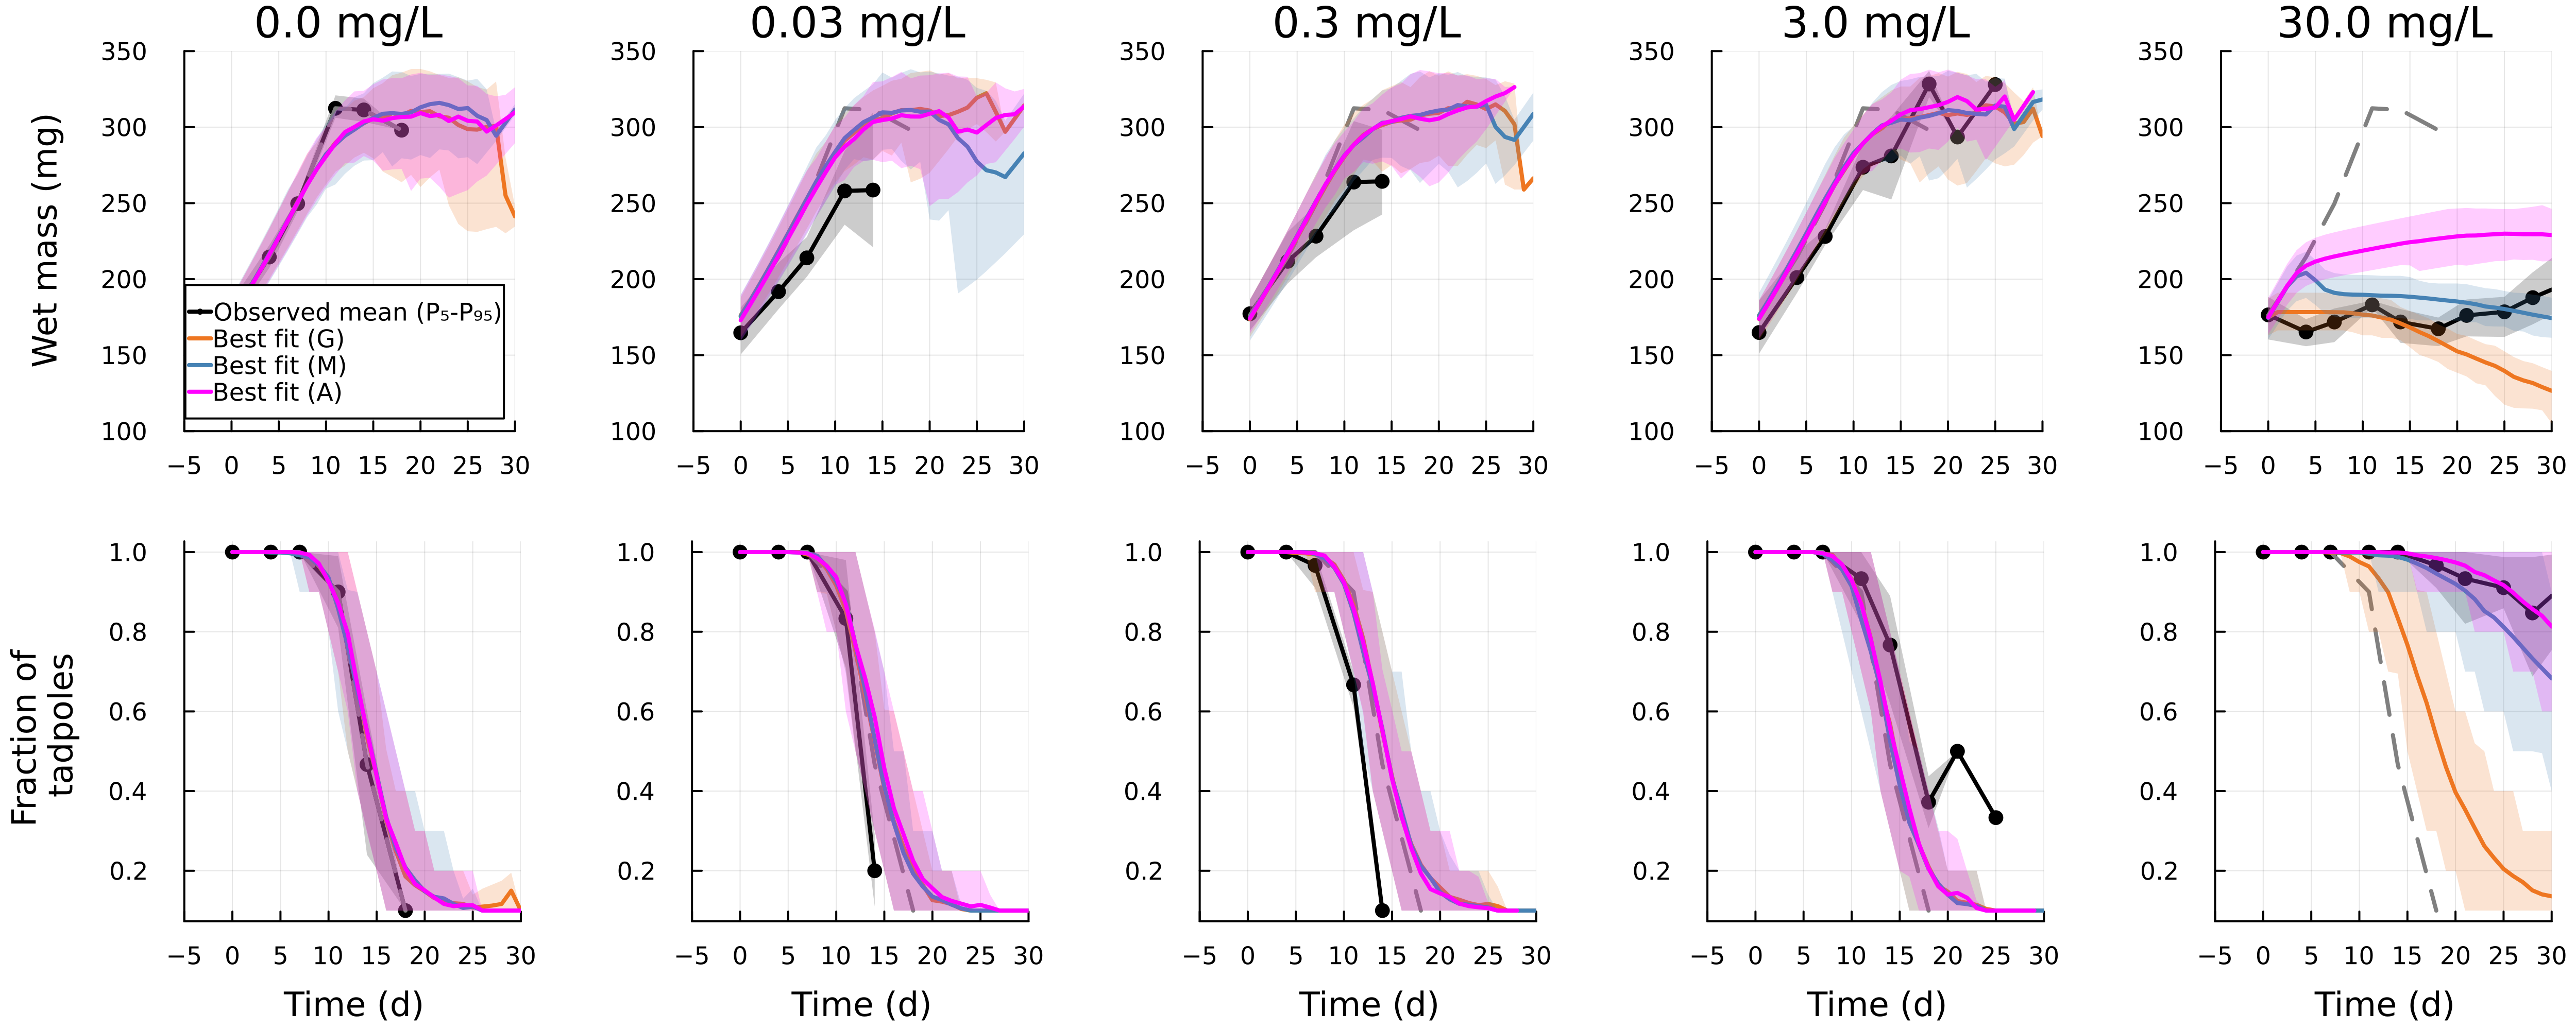
\includegraphics[width=\textwidth]{Discoglossus_24D_summaries_PMoA_comparison.png}
    \caption{
        2,4-D model fit to larval data for different physiological modes of action. 
        Error bands indicate 5th to 95th percentiles. 
        Variability in model output reflects individual variability. 
        Non-monotonicity in the fraction of tadpoles at 3 mg/L is the result of a missing value.
        G = decrease in growth efficiency, M = increase in maintenance costs, A = decrease in assimilation efficiency.
    }
    \label{fig:pmoa_comparison_24d}

\end{figure}

\subsubsection{Effects of Flupyradifurone on larvae}

Flupyradifurone caused effects of growth at 100 mg/L, 
but without a clear delay in metamorphosis. 
Based on the calibration in to 2,4-D data, we could rule out PMoAs $M$ and $A$, 
because both imply a delay in metamorphosis when growth is affected. 
Since the timing of metamorphosis was slightly earlier in the affected treatment, 
we also considered PMoA $\kappa$, which causes increased investment in maturation. 
PMoA $G$ clearly explained effects on growth better, while implying a slight delay in metamorphosis 
(Figure \ref{fig:pmoa_comparison_flp}). 
PMoA $\kappa$ over-predicted the effects on growth, causing severy shrinking at high concentrations, 
while also over-predicting the effects on premature metamorphosis. 
Based on this calibration, PMoA $G$ is more plausible.

\begin{figure}[!htb]
    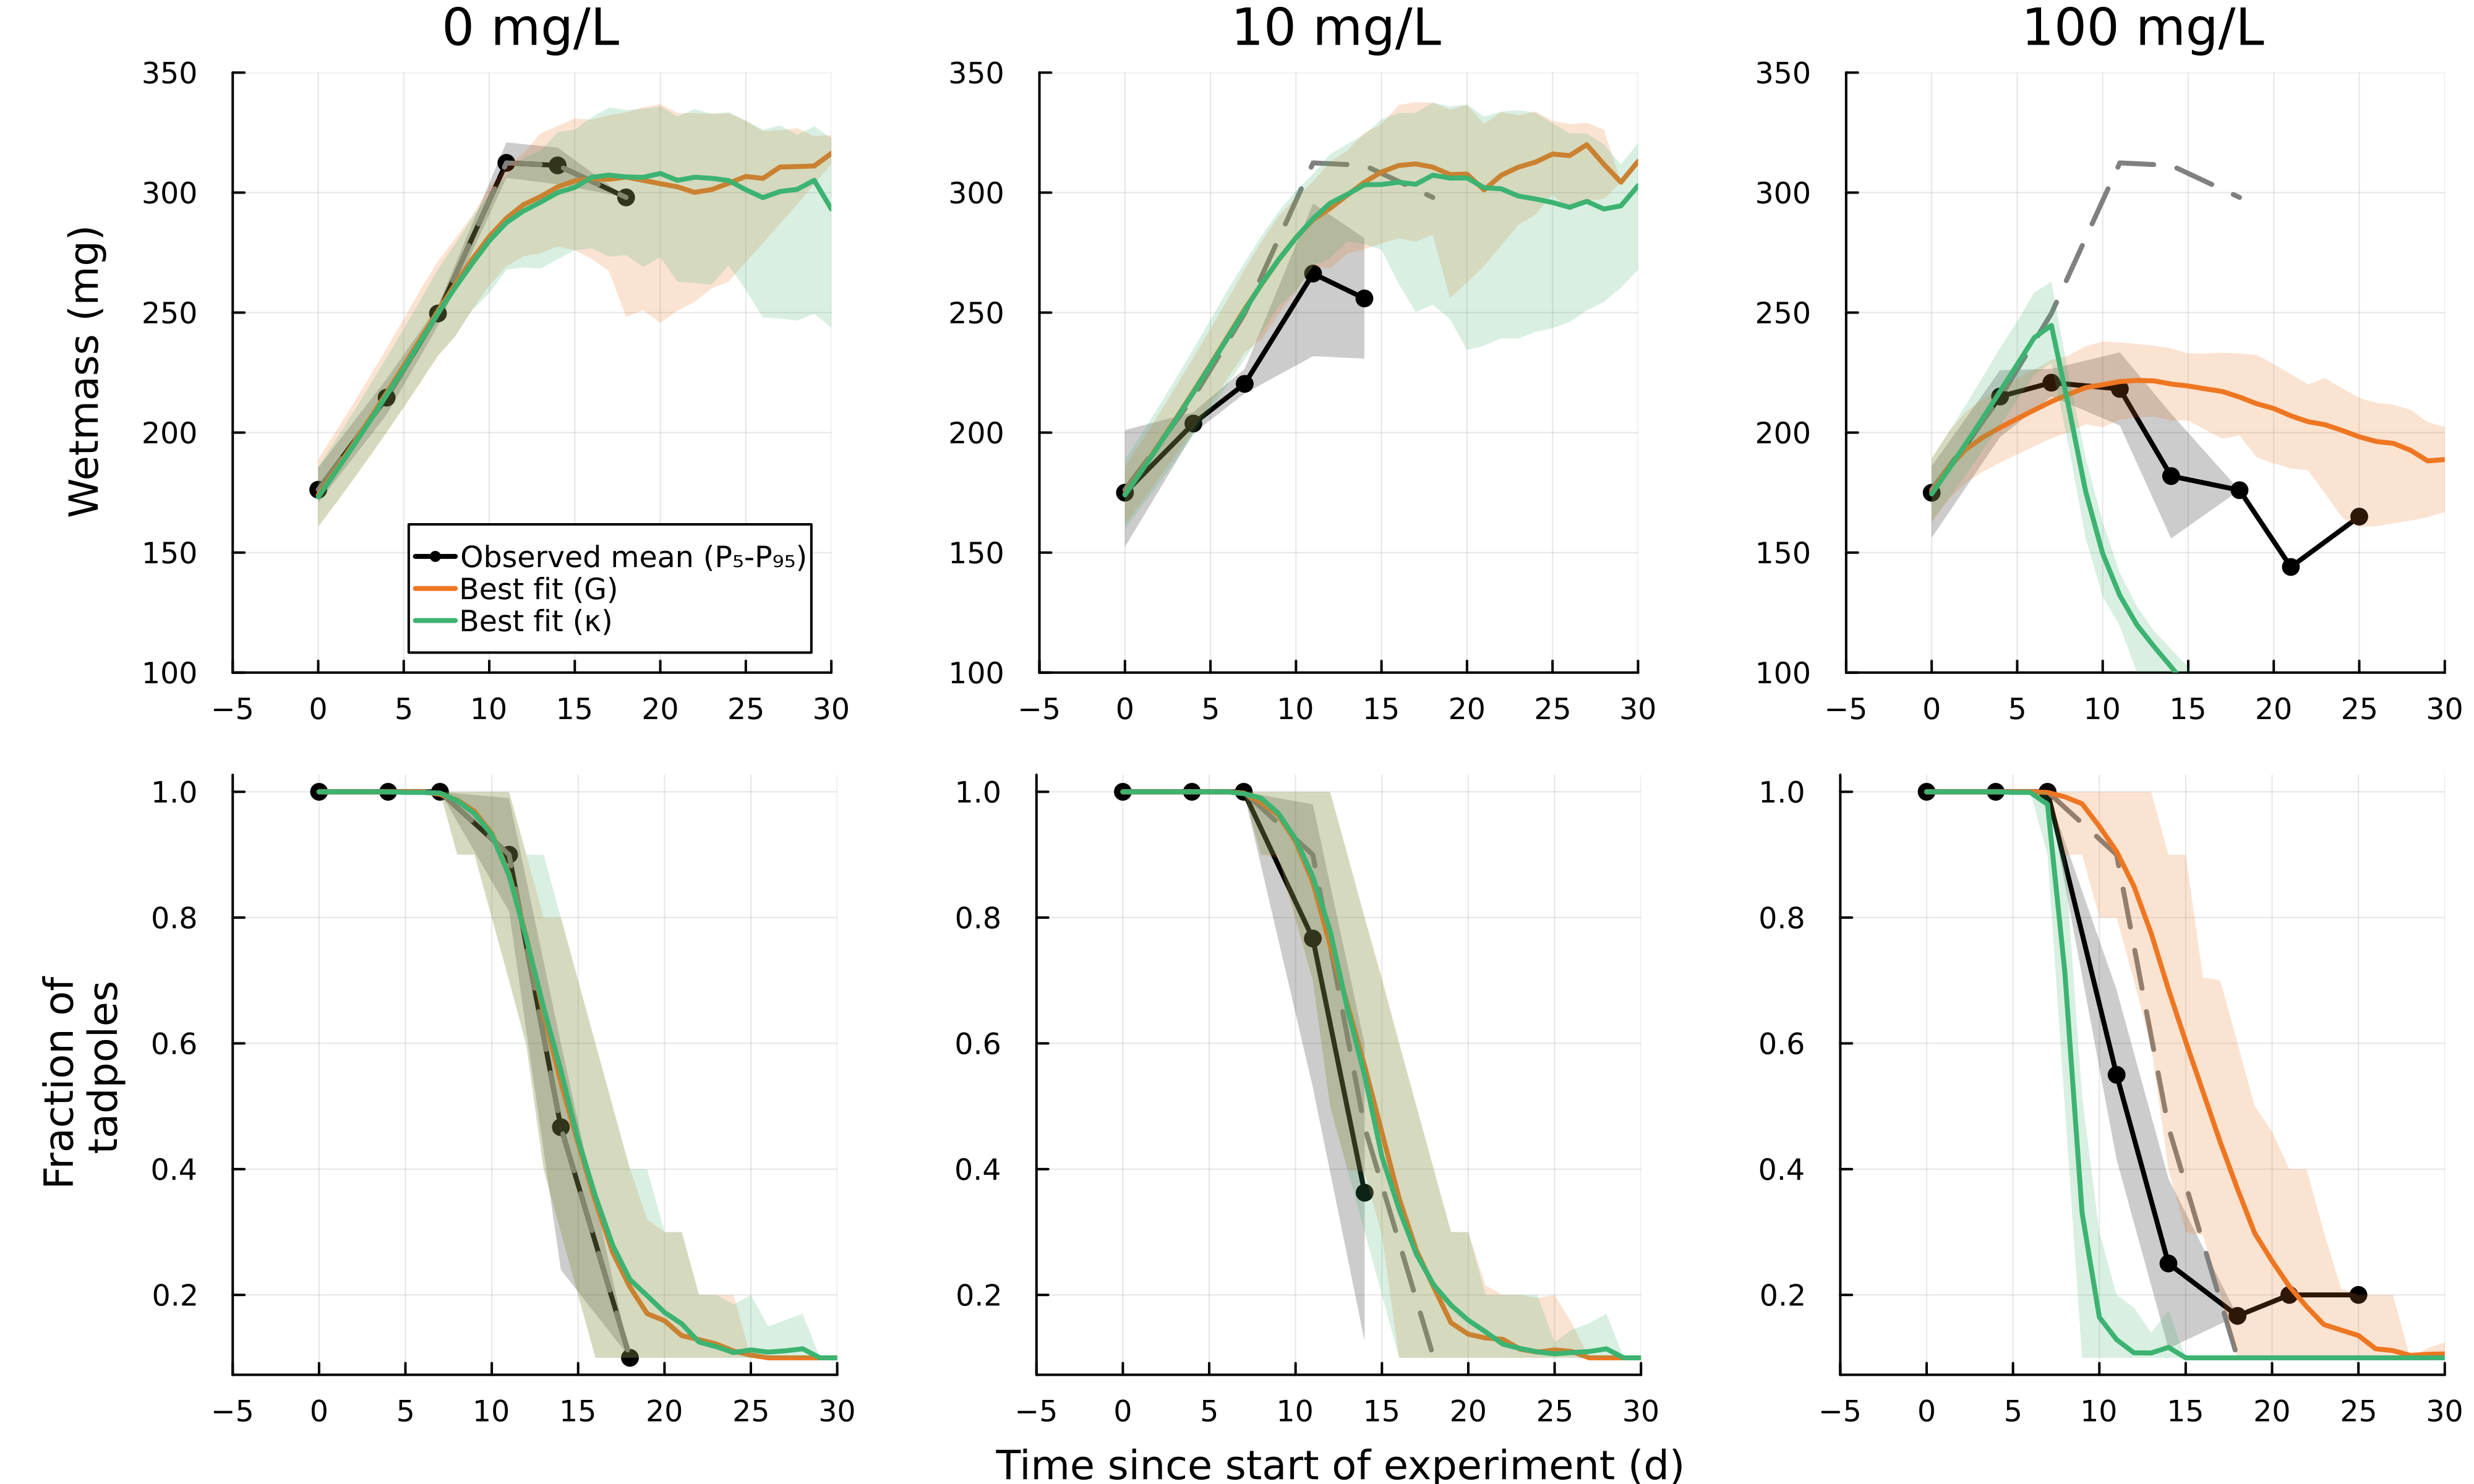
\includegraphics[width=\textwidth]{Discoglossus_Flupyradifurone_summaries_PMoA_comparison.png}
        \caption{
        Flupyradifurone model fit to larval data for different physiological modes of action. 
        Error bands indicate 5th to 95th percentiles. 
        Variability in model output reflects individual variability. 
        G = decrease in growth efficiency, $\kappa$ = decreased resource allocation to growth/increased resource allocation to maturation.
    }
    \label{fig:pmoa_comparison_flp}

\end{figure}

\subsection{Cross-validation: Effects of 2,4-D at GS 46}
2,4-D caused delay of GS 46 and a decrease 
in the mass at GS 46. 
The effect of timing was predicted imprecisely, but accurately. 
The prediction accuracy for the timing of GS 46 was similar for PMoAs $M$ and $A$ (Figure \ref{fig:metamorps_24D}).
Effects on mass at GS 46 were under-predicted by both PMoAs, 
but less so by $M$. 
We  therefore concluded that $M$ is the more plausible PMoA to explain effects of 2,4-D. 
The associated MAPE was 22\% for the timing of GS 46 and 17\% for mass at GS 46. 

\begin{figure}[!htb]
    
\includegraphics[width=\textwidth]{CrossValidation_Discoglossus_24D_PMoA_comparison.png}
    \caption{
        Forward predictions of 2,4-D effects on metamorphosis traits based on two alternative PMoAs. 
        Distributions are plotted as kernel density estimates and show the distributions across individuals. 
        Variability in model output reflects individual variability. 
        M = increase in maintenance costs, A = decrease in assimilation efficiency.  
        G46 = developmental stage gosner stage 46.
        MAPE = mean absolute percent error, calculated only for predictions. 
        }    
    \label{fig:metamorps_24D}
\end{figure}

\subsection{Cross-validation: Effects of Flupyradifurone at GS 46}

Effects of Flupyradifurone on the timing of GS 46 were predicted well by PMoA $G$ (decrease in growth efficiency), but not by $\kappa$ (shift in resource allocation from growth to maturation). 
While both PMoAs correctly predicted the effect on wet mass at GS 46, 
the difference between PMoAs was clearly visible in the predicted effects on the timing of GS 46. 
While we observed no clear effect of Flupyradifurone on the timing of GS 46, 
PMoA $\kappa$ implied that GS 46 would be reached sooner at high exposure concentrations (a shortening of metamorphosis), 
which was not observed. PMoA $G$ correctly predicted that the timing of GS 46 is unaffected by Flupyradifurone exposure (Figure \ref{fig:metamorps_flupy}).
Therefore, we concluded that the effects of Flupyradiforone were more likely caused by a decrease in growth efficiency,
rather than a in the resource allocation from growth to maturation. 

\begin{figure}[!htb]
    
\includegraphics[width=\textwidth]{CrossValidation_Discoglossus_Flupyradifurone_PMoA_comparison.png}
    \caption{
        Forward predictions of Flupyradifurone (Sivanto) effects on metamorphosis traits based on two alternative PMoAs. 
        Distributions are plotted as kernel density estimates and show the distributions across individuals. 
        Variability in model output reflects individual variability. 
        G46 = developmental stage gosner stage 46.
        G = decrease in growth efficiency, $\kappa$ = decreased investment in growth/increased investment in maturation.  
        MAPE = mean absolute percent error = mean relative error, calculated only for predictions. 
        }
    \label{fig:metamorps_flupy}
\end{figure}


\subsection{Model validatiation: Predicting mixture effects}

\subsubsection{Predicting mixture effects on larvae}

Based on the insights from calibration and cross-validation, 
we generated predictions of mixture toxicity by assuming PMoA $M$ for 2,4-D and $G$ for Flupyradifurone. \\
In the mixture treatments, the data indicated a dominance effect of 2,4-D with respect to growth 
and timing of metamorphosis. 
That is, additional exposure to Flupyradifurone did not alter the response to 2,4-D. 
This was predicted accurately by the model (Figure \ref{fig:mixture_growth}, Figure \ref{fig:mixture_fracttadpoles}).
In the highest 2,4-D treatment, the model predicted severe shrinking and a complete inability to reach metamorphosis, 
which is generally in line with the observation that this treamtent caused 100\% mortality.
%
\begin{figure}[!htb]

    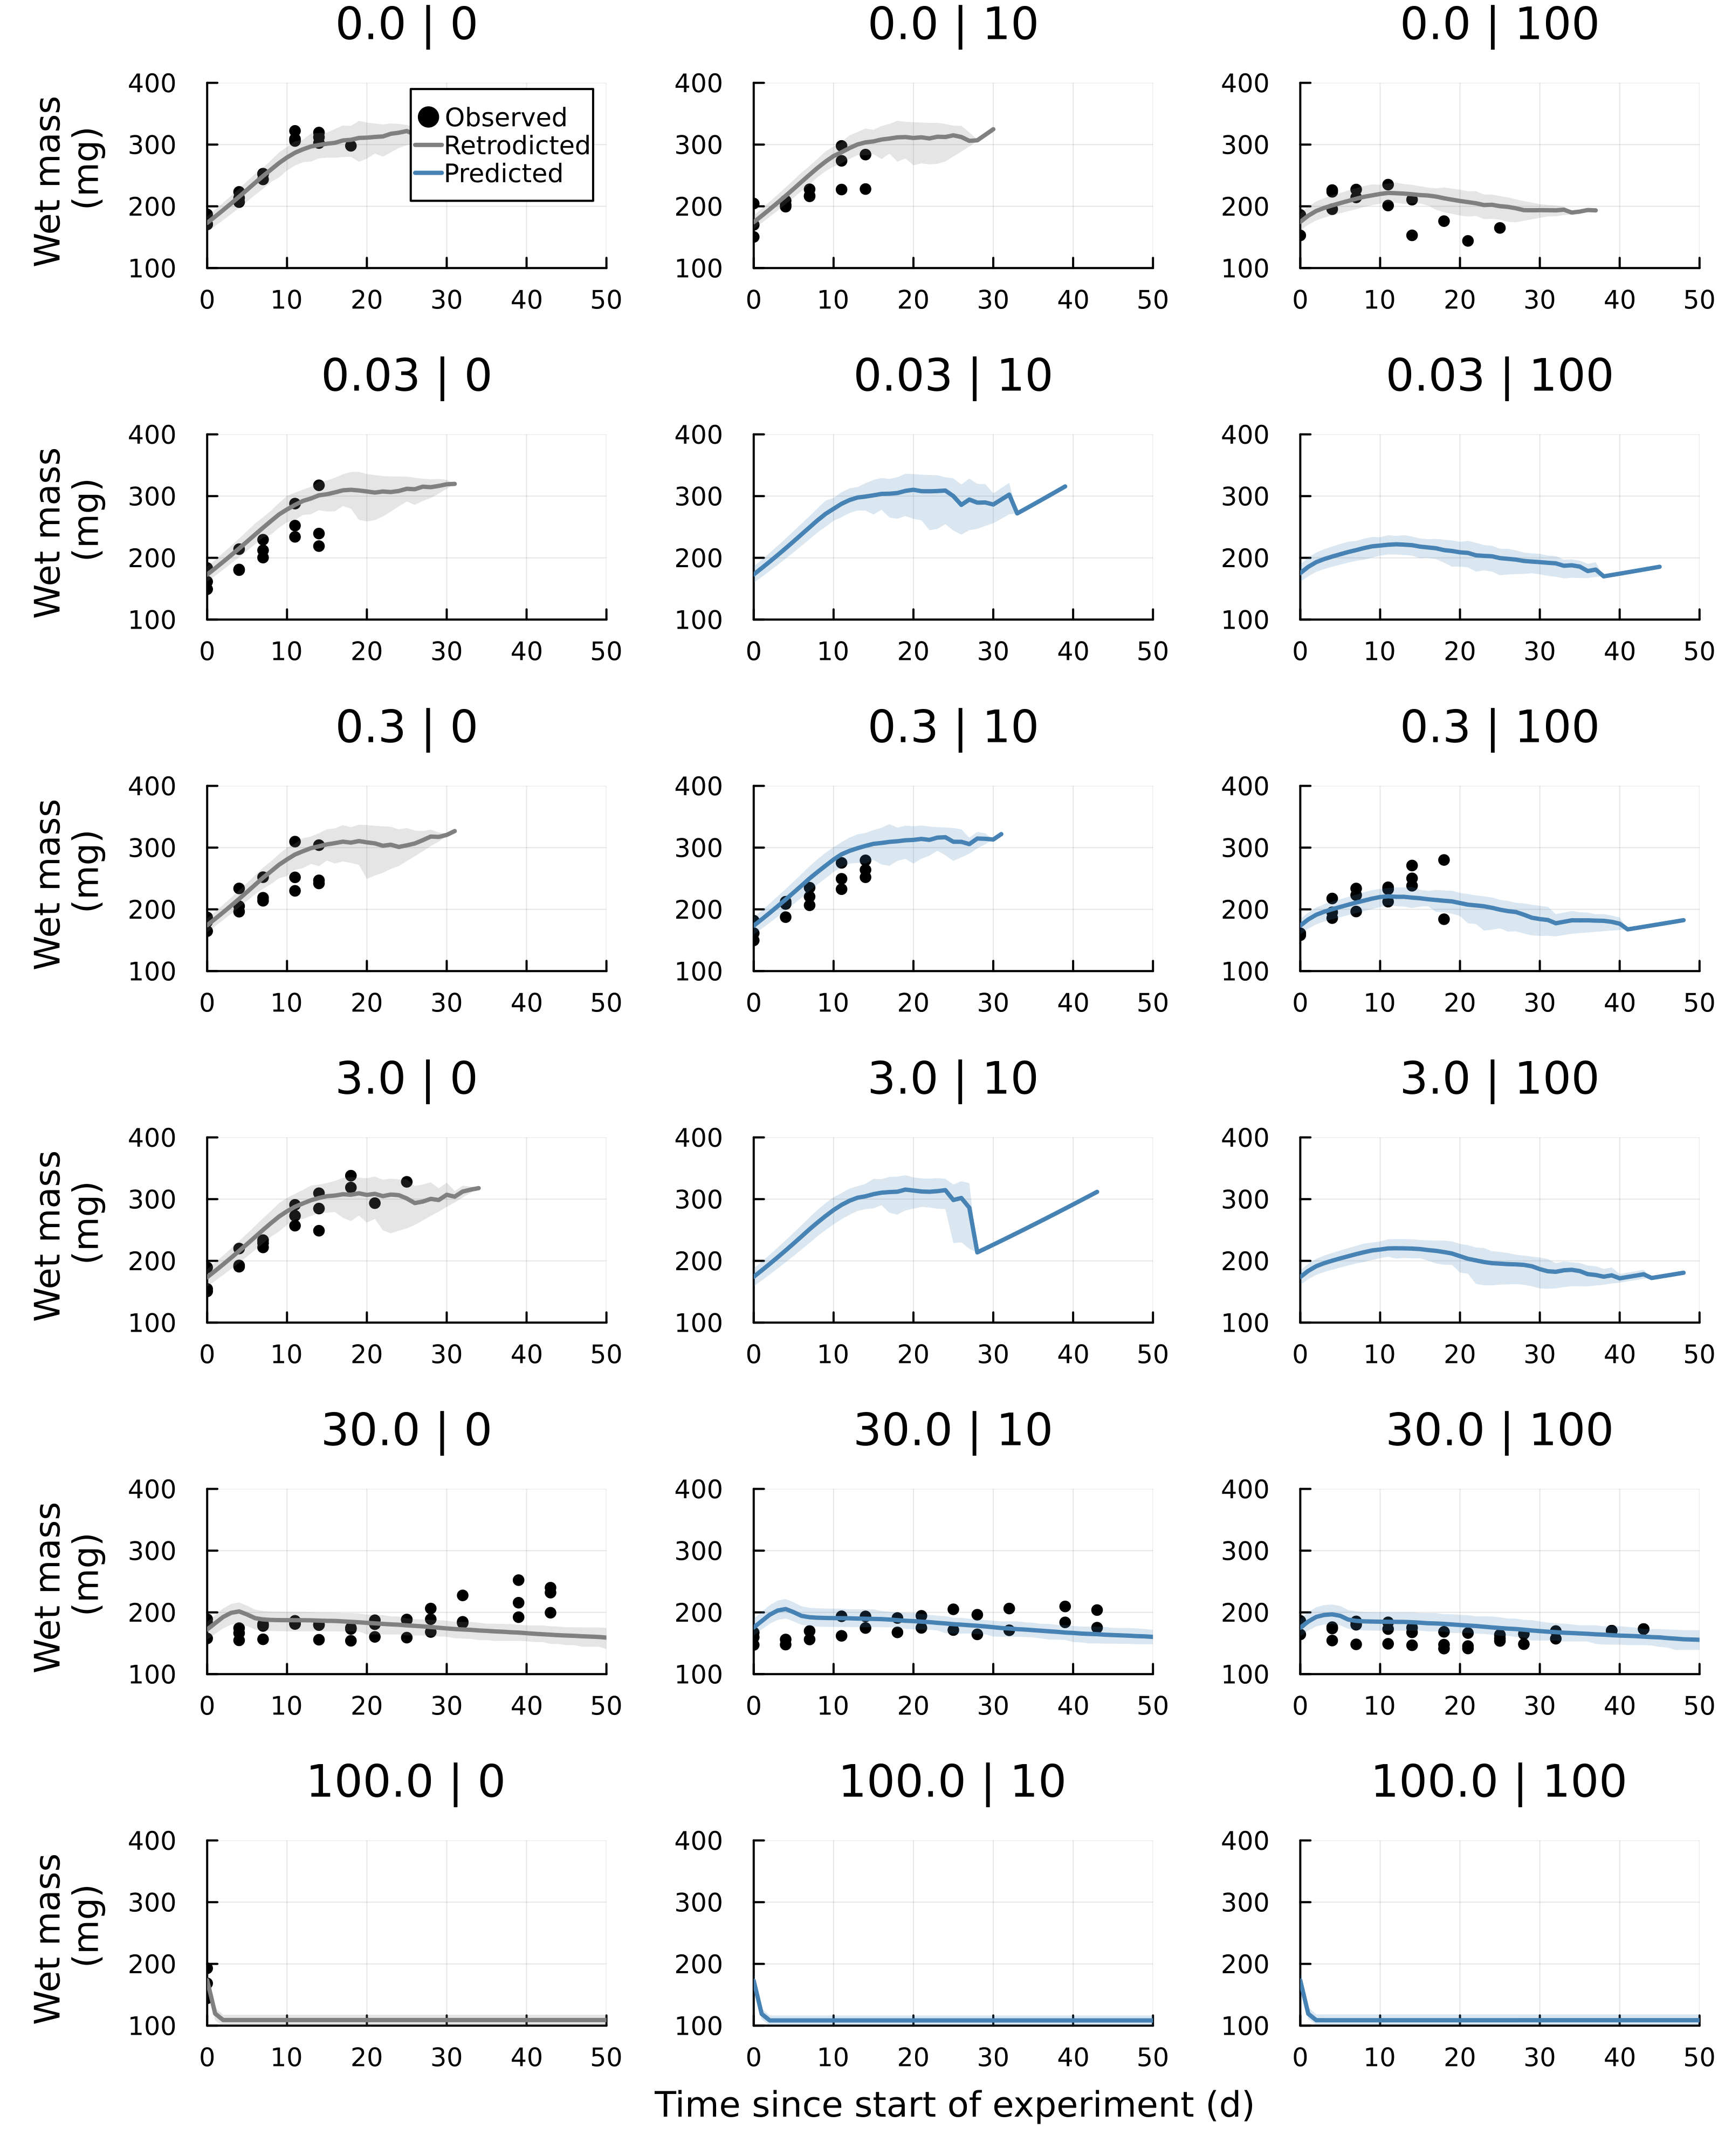
\includegraphics[width=\textwidth]{ModelValidation_Discoglossus_UCLM_mixture_growth.png}
    \caption{
        Forward predictions of binary mixture effects on larval growth. 
        Rows correspond to 2,4-D exposure concentrations, 
        columns to Flupyradifurone exposures (both in $mg/L$).
        Variability in model output reflects individual variability. 
        Error bands indicate 5th to 95th percentiles.
    }
    \label{fig:mixture_growth}
    
\end{figure}
%
\begin{figure}[!htb]
    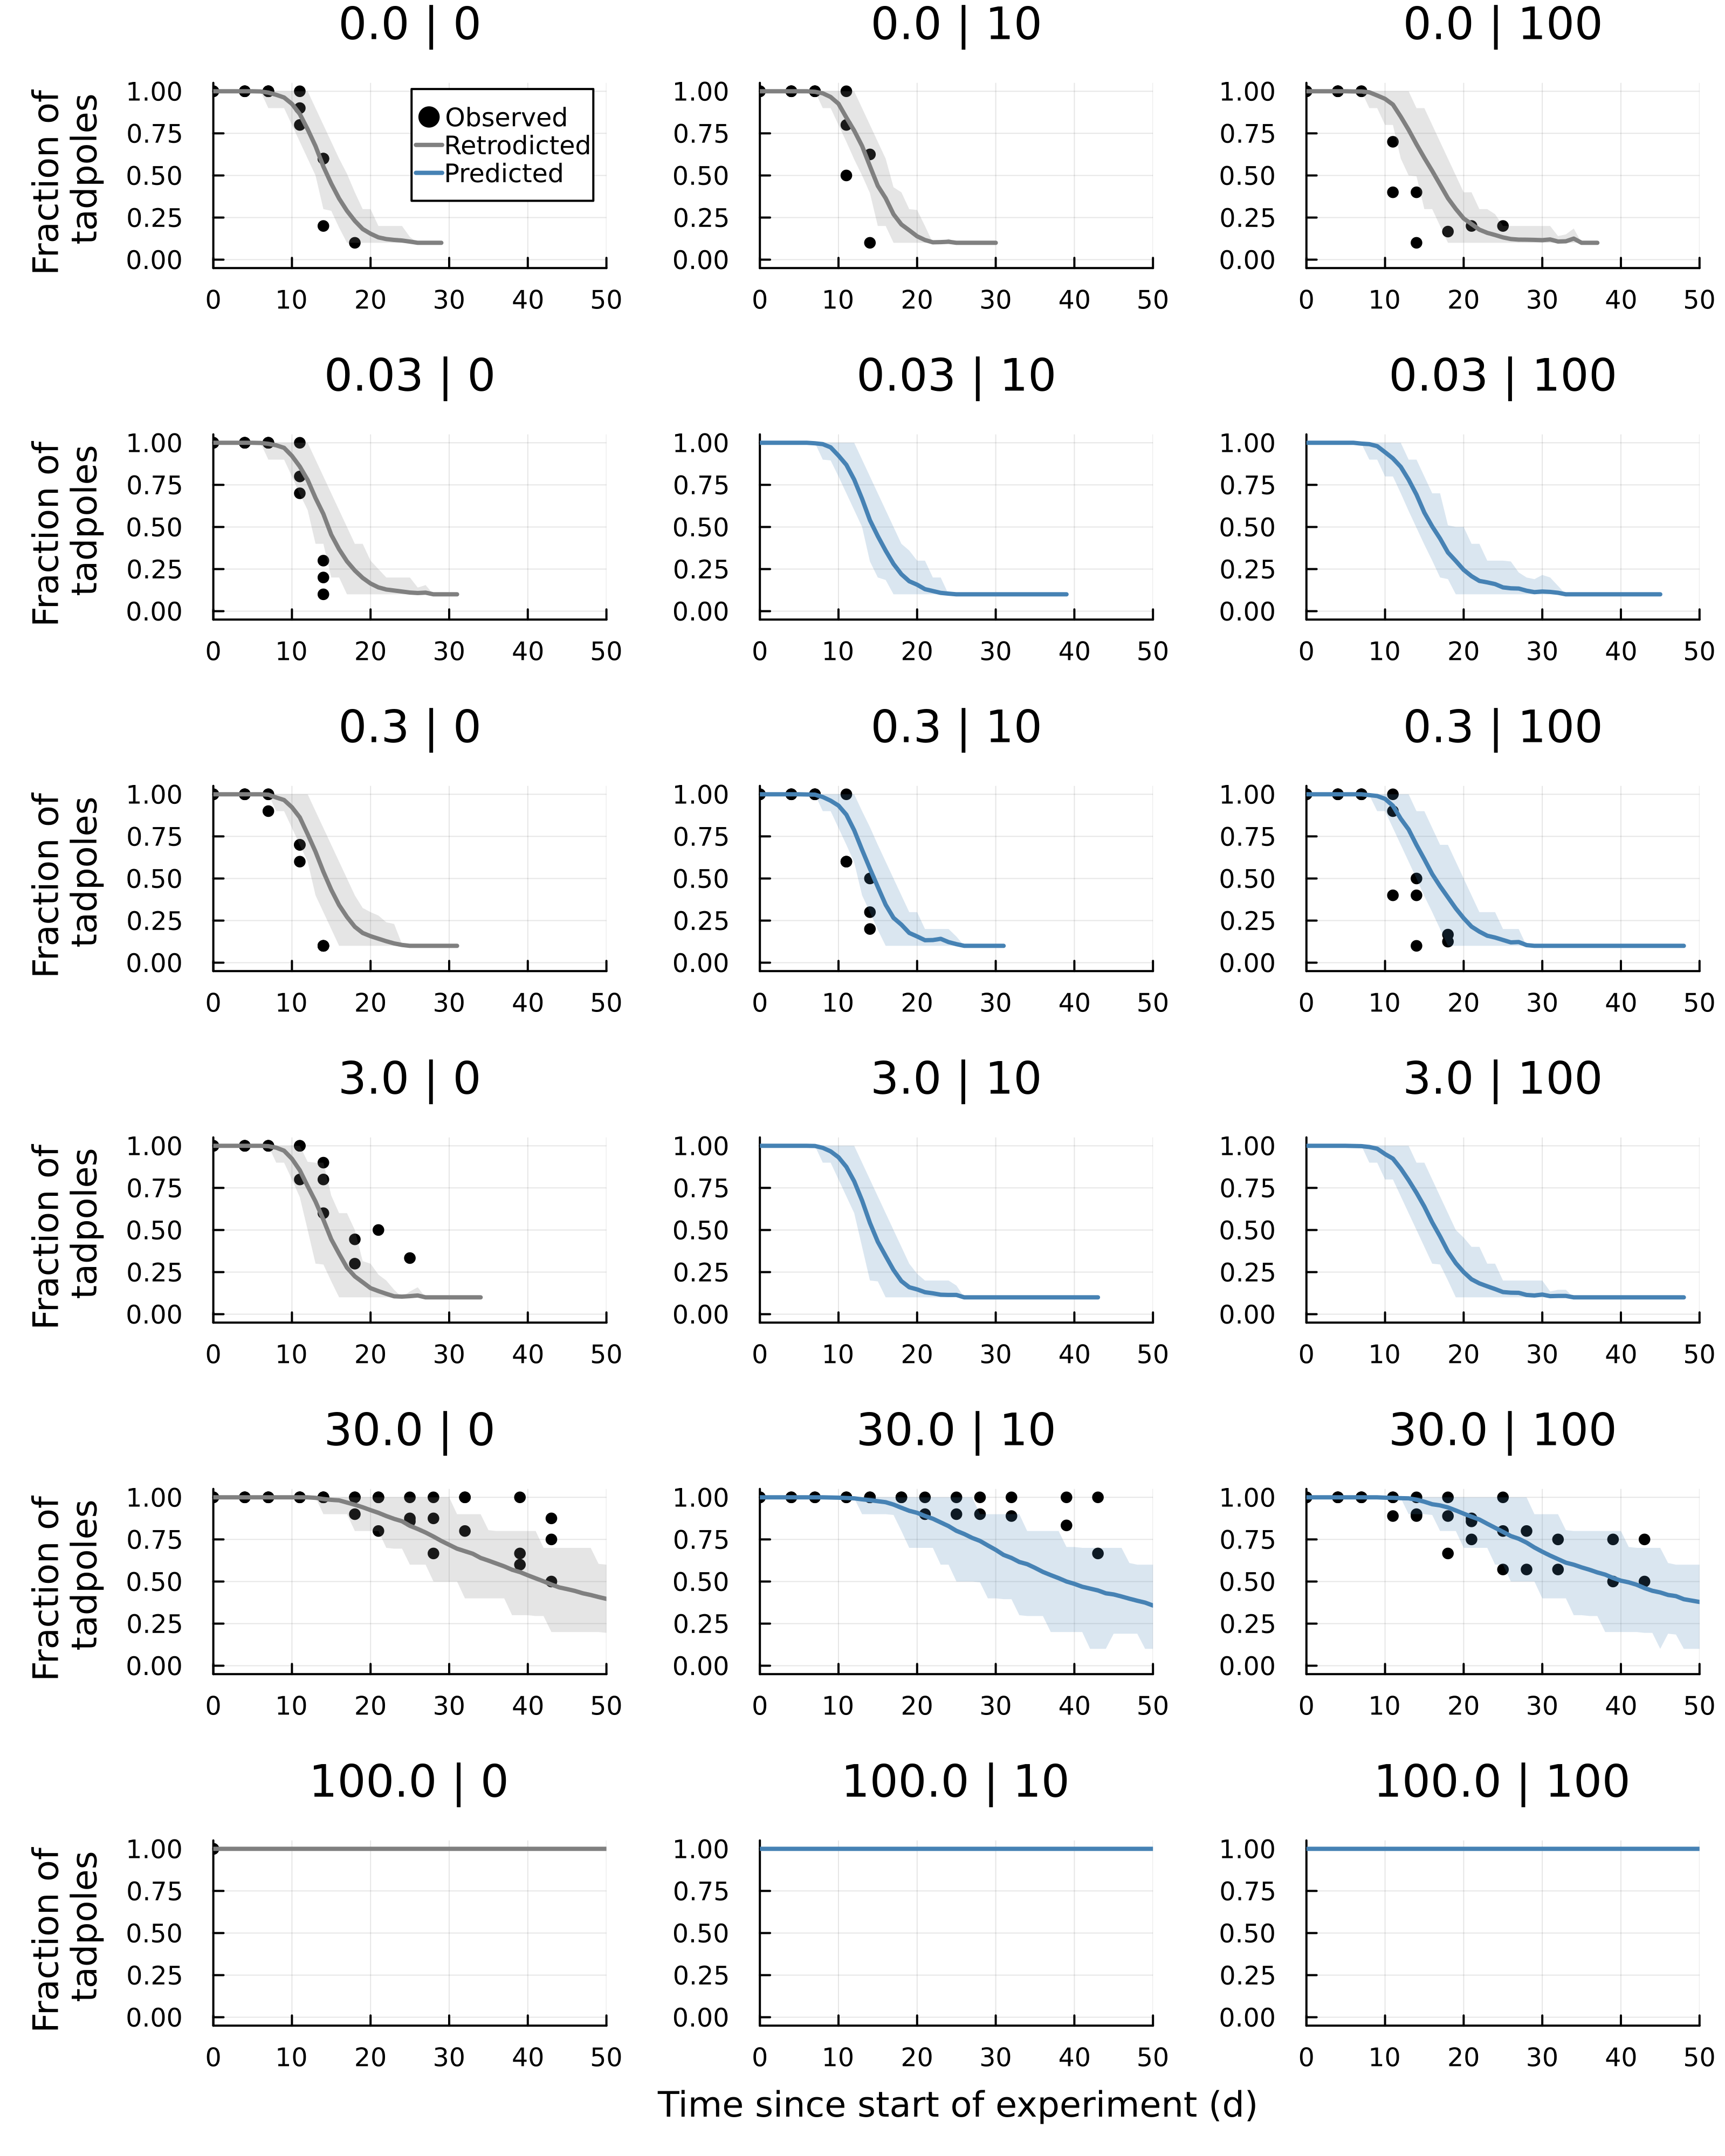
\includegraphics[width=\textwidth]{ModelValidation_Discoglossus_UCLM_mixture_fracttadpoles.png}
    \caption{
        Forward predictions of binary mixture effects on the time to reach metamorphosis (Gosner stage 42).
        \textit{Fraction of tadpoles} is the number of test organisms which have not yet reached metamorphosis, 
        relative to the total number of surviving individuals. \\ 
        Rows correspond to 2,4-D exposure concentrations, 
        columns to Flupyradifurone exposures (both in $mg/L$).
        Variability in model output reflects individual variability. 
        Error bands indicate 5th to 95th percentiles.
    }
    \label{fig:mixture_fracttadpoles}
    
\end{figure}
%
\subsubsection{Predicting mixture effects on metamorphs}
%
Similarly to the result of the cross-validation, the model predicted 
mixture effects on the timing of GS 46 with high accuracy, but low accuracy (Figure \ref{fig:mixture_metamorphs}). 
This coincided with a high mortality at the corresponding treatments. 
The model predictions imply that individuals, if they would not have died from the epxosure, 
may have taken a long time to complete metamorphosis, given that they reach GS 42 at all. 
Remarkably, the predicted variability in the timing of GS 46 was exclusively the result 
of the simulated individual variability, with the degree of variability estimated from control data \citep{hansulDynamicEnergyBudget2026}.
This is different from the potential variability in simulation outputs that could result from the propagation of parameter uncertainty. \\
The model under-predicted the effects on mass at GS 46 at the higher mixture treatment. 
When we compare this to the predictions of single-stressor effects, 
it becomes apparent that this mostly reflects a tendency of the model to under-predict effects on mass at GS 46, 
rather than under-predict the mixture effect.

\begin{figure}[!htb]
    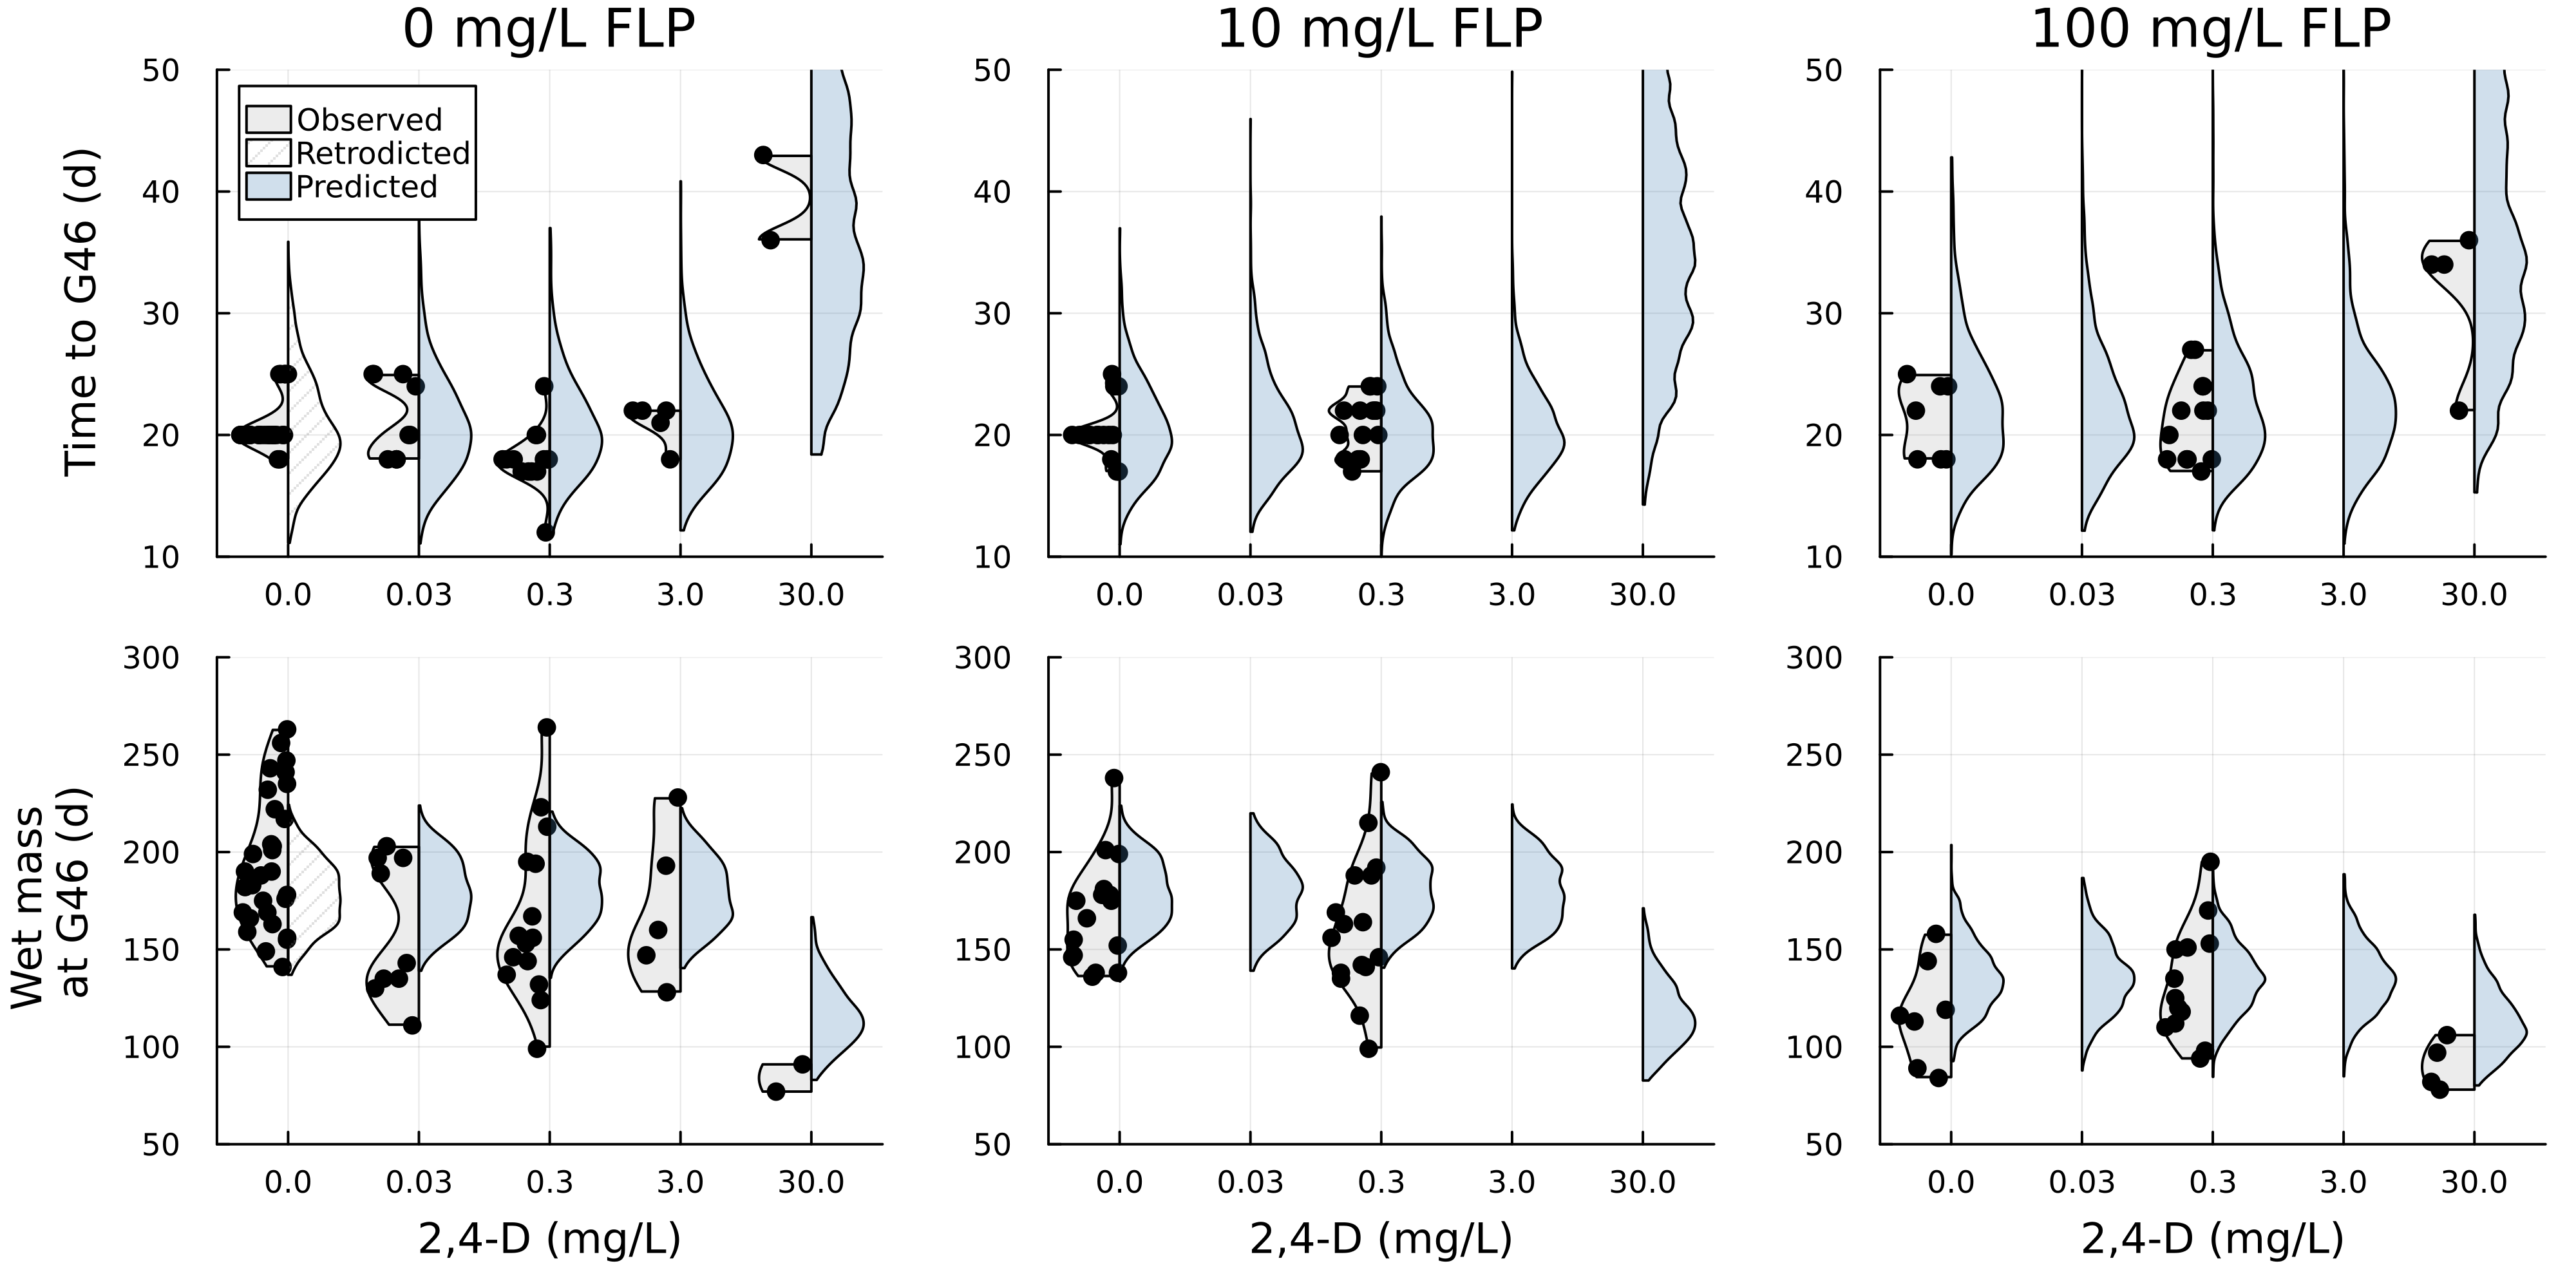
\includegraphics[width=\textwidth]{ModelValidation_Discoglossus_UCLM_mixture_metamorphs.png}
    \caption{
        Predicted effects of Flupyradifurone/Sivanto and 2,4-D on metamorphosis traits. 
        Error bands indicate 5th to 95th percentiles. 
        Variability in model output reflects individual variability. 
        G46 = GS 46. FLP = Flupyradifurone.  
    }
    \label{fig:mixture_metamorphs}
\end{figure}

\section{Discussion}

\subsection{Calibration and cross-validation: Inference of PMoAs from life-history data}
\noindent
By fitting alternative PMoAs to effect data for larvae, 
we could draw some conclusions regarding the plausibility of PMoAs. 
For a given effect on growth, 
PMoAs $M$ and $A$ are associated with a clear delay of metamorphosis, 
whereas PMoA $G$ only implies a subtle delay of metamorphosis. 
This can be explained by the interaction of these PMoAs with mass fluxes in the DEB model.\\
PMoA $G$, i.e. a decrease in growth efficiency, 
only causes an indirect effect on the maturation rate.
Furthermore, any reduction in growth also reduces maintenance costs, 
and the effect of $G$ approaches zero as an individual reaches its maximum length 
(the growth efficiency $\eta_{AS}$ does not affect the equilibrium conditions of the model).
PMoAs $M$ and $A$ on the other hand have a direct effect on growth and maturation.\\
PMoA $\kappa$ represent a special case, as it does not imply a loss of energy, 
but only a change in the allocation of energy. 
In the present study, $\kappa$ did not explain observed effects. 
Generally, a decrease in $\kappa$ might be a plausible candidate if premature metamorphosis is observed 
in combination with adverse effects on growth.\\
The prediction of effects at GS 46 depended heavily on the choice of PMoA. 
The message here is two-fold: 
At the one hand, extrapolations from larval effect data to GS 46 should be done with caution. 
We suggest a model averaging approach if the PMoA identification from larval data is ambiguous.
At the other hand, effect data at GS 46 apparently carries a lot of information regarding the PMoA. 
Generating such effect data is resource-intensive, but for cases where an unequivocal PMoA identification is crucial, 
it could be worth the effort. 
%
\subsection{Validation: Predicting mixture effects}
\noindent
The dominance effect of 2,4-D over Flupyradifurone could be predicted with high accuracy. 
Given that the substances acted via differnt PMoAs, a diferentiation between IA and DA models was obsolete. 
The presence of a dominance effect can be explained through the combination of PMoAs, 
based on the same rationale that was used to select the PMoAs in the first place. 
We identified $G$ as most likely PMoA for Flupyradifurone, 
implying that effects weaken over time and only indirect effects on maturation. 
We identified $M$ as most likely PMoA for 2,4-D, 
implying effects across the entire growth curve, as well as direct effects on the maturation rate. 
%
\subsection{Implications for ampibian population dynamics}
\noindent
While the present study focussed on the modelling of sublethal effects on the individual level, 
one of the goals of the amphibian DEB-TKTD model development is to extrapolate effects to the population level.
Achieving this would at least require that the present analysis is extended to also account for lethal effects. 
In fact, the severity of lethal effects is highly life stage-specific \citep{gonzalez-lopezChronicExposurePesticides2026}, 
with the highest mortality rate ocurring during metamorphosis, 
manifesting metamorphosis as a bottleneck in the amphibian life history.\\ 
Apart from direct lethal effects, the ecology of amphibians implies that sublethal effects in laboratory tests 
may translate to letahl effects in the field.\\
In ephemeral wetlands such as those inhabited by \textit{D. galganoi},
a delay in metamorphosis could lead to death if individuals fail to reach metamorphosis 
before the aquatic habitat has dried out. 
This means that the results presented in the present study could lead 
to dramatically different effects on population dynamics if the effect of drying is considered. 
Simultaneously, it is known that amphibians may accelerate development under drying conditions, 
counter-acting the effects described here. 
Such acceleration of development may in turn lead to adverse effects in later life stages. 
These are relationships between chemical exposure and amphibian life-history that have not been considered 
in the present study, but could be integrated into a DEB-TKTD modelling approach.
%
\subsection{Conclusions}
\noindent 
We have demonstrated that DEB-TKTD models can be used to perform predictive modelling 
of pesticide effects in amphibian larvae and metamorphs.
The extrapolation of effects across life stages depends heavily on the selection of the PMoA. 
DEB-TKTD models can be fitted to larval data up to GS 42 and some inference about the PMoA can be made, 
but data on effects at GS 46 is highly informative regarding the PMoA.
Generally, the model has a tendency to under-predict effects on the mass at metamorphosis. 
The effects of a binary mixture of pesticides with different PMoAs could be predicted with high accuracy.

\clearpage
\appendix
\section{Appendix}

\renewcommand{\thetable}{A\arabic{table}}
\setcounter{table}{0}

\begin{table}[h]
    \caption{Parameter of the physiological baseline model estimated from the control data. 
    Best fit was the value associated with the smallest error in the calibration and used for simulation.
    Median refers to the median of the posterior distribution, $P_{05}$ and $P_{95}$ refer to the 5th to 95th percentiles 
    (credible intervals).
    For further details, see \citet{hansulDynamicEnergyBudget2026}.}
    \label{tab:deb_params}
    \begin{tabular}{ccccc}
    Parameter & Best fit & Median & $P_{05}$ & $P_{95}$\\
    \hline
    $\sigma_{Z,M}$ & 0.153 & 0.252 & 0.16 & 0.304\\
    $\{ \dot{I} \}_{max}$ & 1.79 & 1.61 & 1.38 & 1.86\\
    $k_M^{emb}$ & 0.213 & 0.175 & 0.135 & 0.242\\
    $\eta_{AS}$ & 0.78 & 0.878 & 0.62 & 0.979\\
    $H^{j}$ & 9.11 & 12.3 & 7.01 & 18.9\\
    $\gamma$ & 0.829 & 0.718 & 0.564 & 0.828\\
    $k_J$ & 0.0088 & 0.0117 & 0.00104 & 0.0408\\
    $\kappa$ & 0.81 & 0.739 & 0.67 & 0.857\\
    $Larval\ water\ content$ & 0.935 & 0.94 & 0.934 & 0.946\\
    $Juvenile\ water\ content$ & 0.892 & 0.864 & 0.792 & 0.906\\
    $Time\ since\ birth$ & 23.5 & 20.6 & 16.7 & 24.3\\
    \end{tabular}
\end{table}

%\label{app1}

%% For citations use: 
%%       \citet{<label>} ==> Lamport [21]
%%       \citep{<label>} ==> [21]
%%


%% If you have bib database file and want bibtex to generate the
%% bibitems, please use
%%
%%  \bibliographystyle{elsarticle-num-names} 
%%  \bibliography{<your bibdatabase>}

%% else use the following coding to input the bibitems directly in the
%% TeX file.

%% Refer following link for more details about bibliography and citations.
%% https://en.wikibooks.org/wiki/LaTeX/Bibliography_Management

\bibliographystyle{elsarticle-harv}
\bibliography{PredictiveModellingChemicalToxicity}
\end{document}

\endinput
%%
%% End of file `elsarticle-template-num-names.tex'.
